\documentclass[11pt, a4paper]{article}

\usepackage{graphicx} % Para insertar imágenes
\usepackage[spanish, english]{babel} 
\usepackage{amsfonts, amsmath, amssymb} % Símbolos matemáticos
\usepackage{float}
\usepackage{setspace}
\usepackage{hyperref} % Referencias
\usepackage{caption} % Poner captione en el medio 
\usepackage{mwe} % for blindtext and example-image-a in example
\usepackage{wrapfig}

% Reference settings
\hypersetup{
    colorlinks=true,
    linkcolor=black,
    filecolor=magenta,      
    urlcolor=blue,
    citecolor=black,
    pdftitle={TP2 - Espectro solar - Cavalieri y Chen},
    pdfpagemode=FullScreen,
}


% Título
\title{TP 2 - Astronomía\\Obtención y análisis del espectro de la luz solar}
\author{Ian Chen y Lola Cavalieri}
\date{15 de octubre de 2024}


%%%%%%%%%%%%%%%%%%%%%%%%%%%%%%%%%%%%%%%%
\begin{document}
% Primera página
\maketitle
\selectlanguage{spanish}
\begin{abstract}
En este trabajo capturamos y analizamos el espectro solar para identificar elementos y estimar la temperatura superficial del Sol. La imagen se tomó en formato RAW y se procesó en \textit{Annie} para obtener un gráfico de intensidad en función de la longitud de onda. Calibramos el espectro utilizando dos picos conocidos: $4861 \AA$ ($H-\beta$) y 5167 Å ($Mg\ I$).  

Identificamos varios elementos, como $Fe\ I$, \textit{Mg I}, \textit{Na I} y \textit{H}, comparando las líneas de absorción con el Solar Flux Atlas. Aplicando la Ley de Wien, calculamos una temperatura de $5392,94 \, \pm \, 19,15$ K, coherente con la clasificación del Sol como estrella G2V.  

Finalmente, comparamos nuestros resultados con datos profesionales y de otro grupo experimental, observando que las diferencias se debieron a variaciones en la captura. Además, realizamos un ajuste con la Ley de Planck para modelar la radiación solar como un cuerpo negro ideal.

\end{abstract}


\selectlanguage{english}
\begin{abstract}
In this work, we captured and analyzed the solar spectrum to identify elements and estimate the Sun's surface temperature. The image was taken in RAW format and processed in \textit{Annie} to obtain an intensity graph as a function of wavelength. The spectrum was calibrated using two known peaks: $4861 \AA$ ($H-\beta$) and 5167 Å ($Mg\ I$).  

We identified several elements, such as $Fe\ I$, \textit{Mg I}, \textit{Na I}, and \textit{H}, by comparing the absorption lines with the Solar Flux Atlas. Using Wien's Law, we calculated a temperature of $5392.94 \, \pm \, 19.15$ K, consistent with the classification of the Sun as a G2V star.  

Finally, we compared our results with professional data and those from another experimental group, observing that the differences were due to variations in the capture process. Additionally, we applied Planck’s Law to model the solar radiation as an ideal black body.

\end{abstract}

\selectlanguage{spanish}
\newpage
%----------------------
\section{Introducción}
En este trabajo analizamos el espectro de la luz del Sol para extraer información relevante, como por ejemplo de qué está hecho y cuál es su temperatura superficial. Para entender este proceso, es importante conocer algunos conceptos básicos de física, química y astronomía 

Primero, cuando la luz emitida por un objeto pasa a través de gases o elementos en su superficie, ciertos colores específicos se absorben, creando líneas de absorción en el espectro. Como cada elemento genera ciertas líneas de absorción específicas, se pueden identificar los elementos circundantes de la fuente de emisión, objeto de estudio de la espectroscopia.

Las estrellas se clasifican en clases espectrales (O, B, A, F, G, K, M) según su temperatura superficial, siendo las de tipo O las más calientes y las de tipo M las más frías. El Sol pertenece a la clase G2V, lo que indica que es una estrella amarilla con una temperatura superficial aproximada de entre 5.000 K y $6.000$ K.  

En este análisis también aplicamos leyes fundamentales como la Ley de Wien, que permite calcular la temperatura de un cuerpo en función de la longitud de onda en la que emite su máxima energía, y la Ley de Planck, que describe cómo un cuerpo ideal (llamado cuerpo negro) emite radiación en función de su temperatura.  

Con estos conceptos en mente, estudiamos cómo la luz solar capturada se puede traducir en un gráfico de intensidades para identificar elementos y estimar la temperatura del Sol, comparando nuestros resultados con datos obtenidos por fuentes científicas profesionales. 

%-----------------------------------
\section{Procedimiento experimental}
\begin{wrapfigure}{1}{0.5\textwidth}
    \centering
    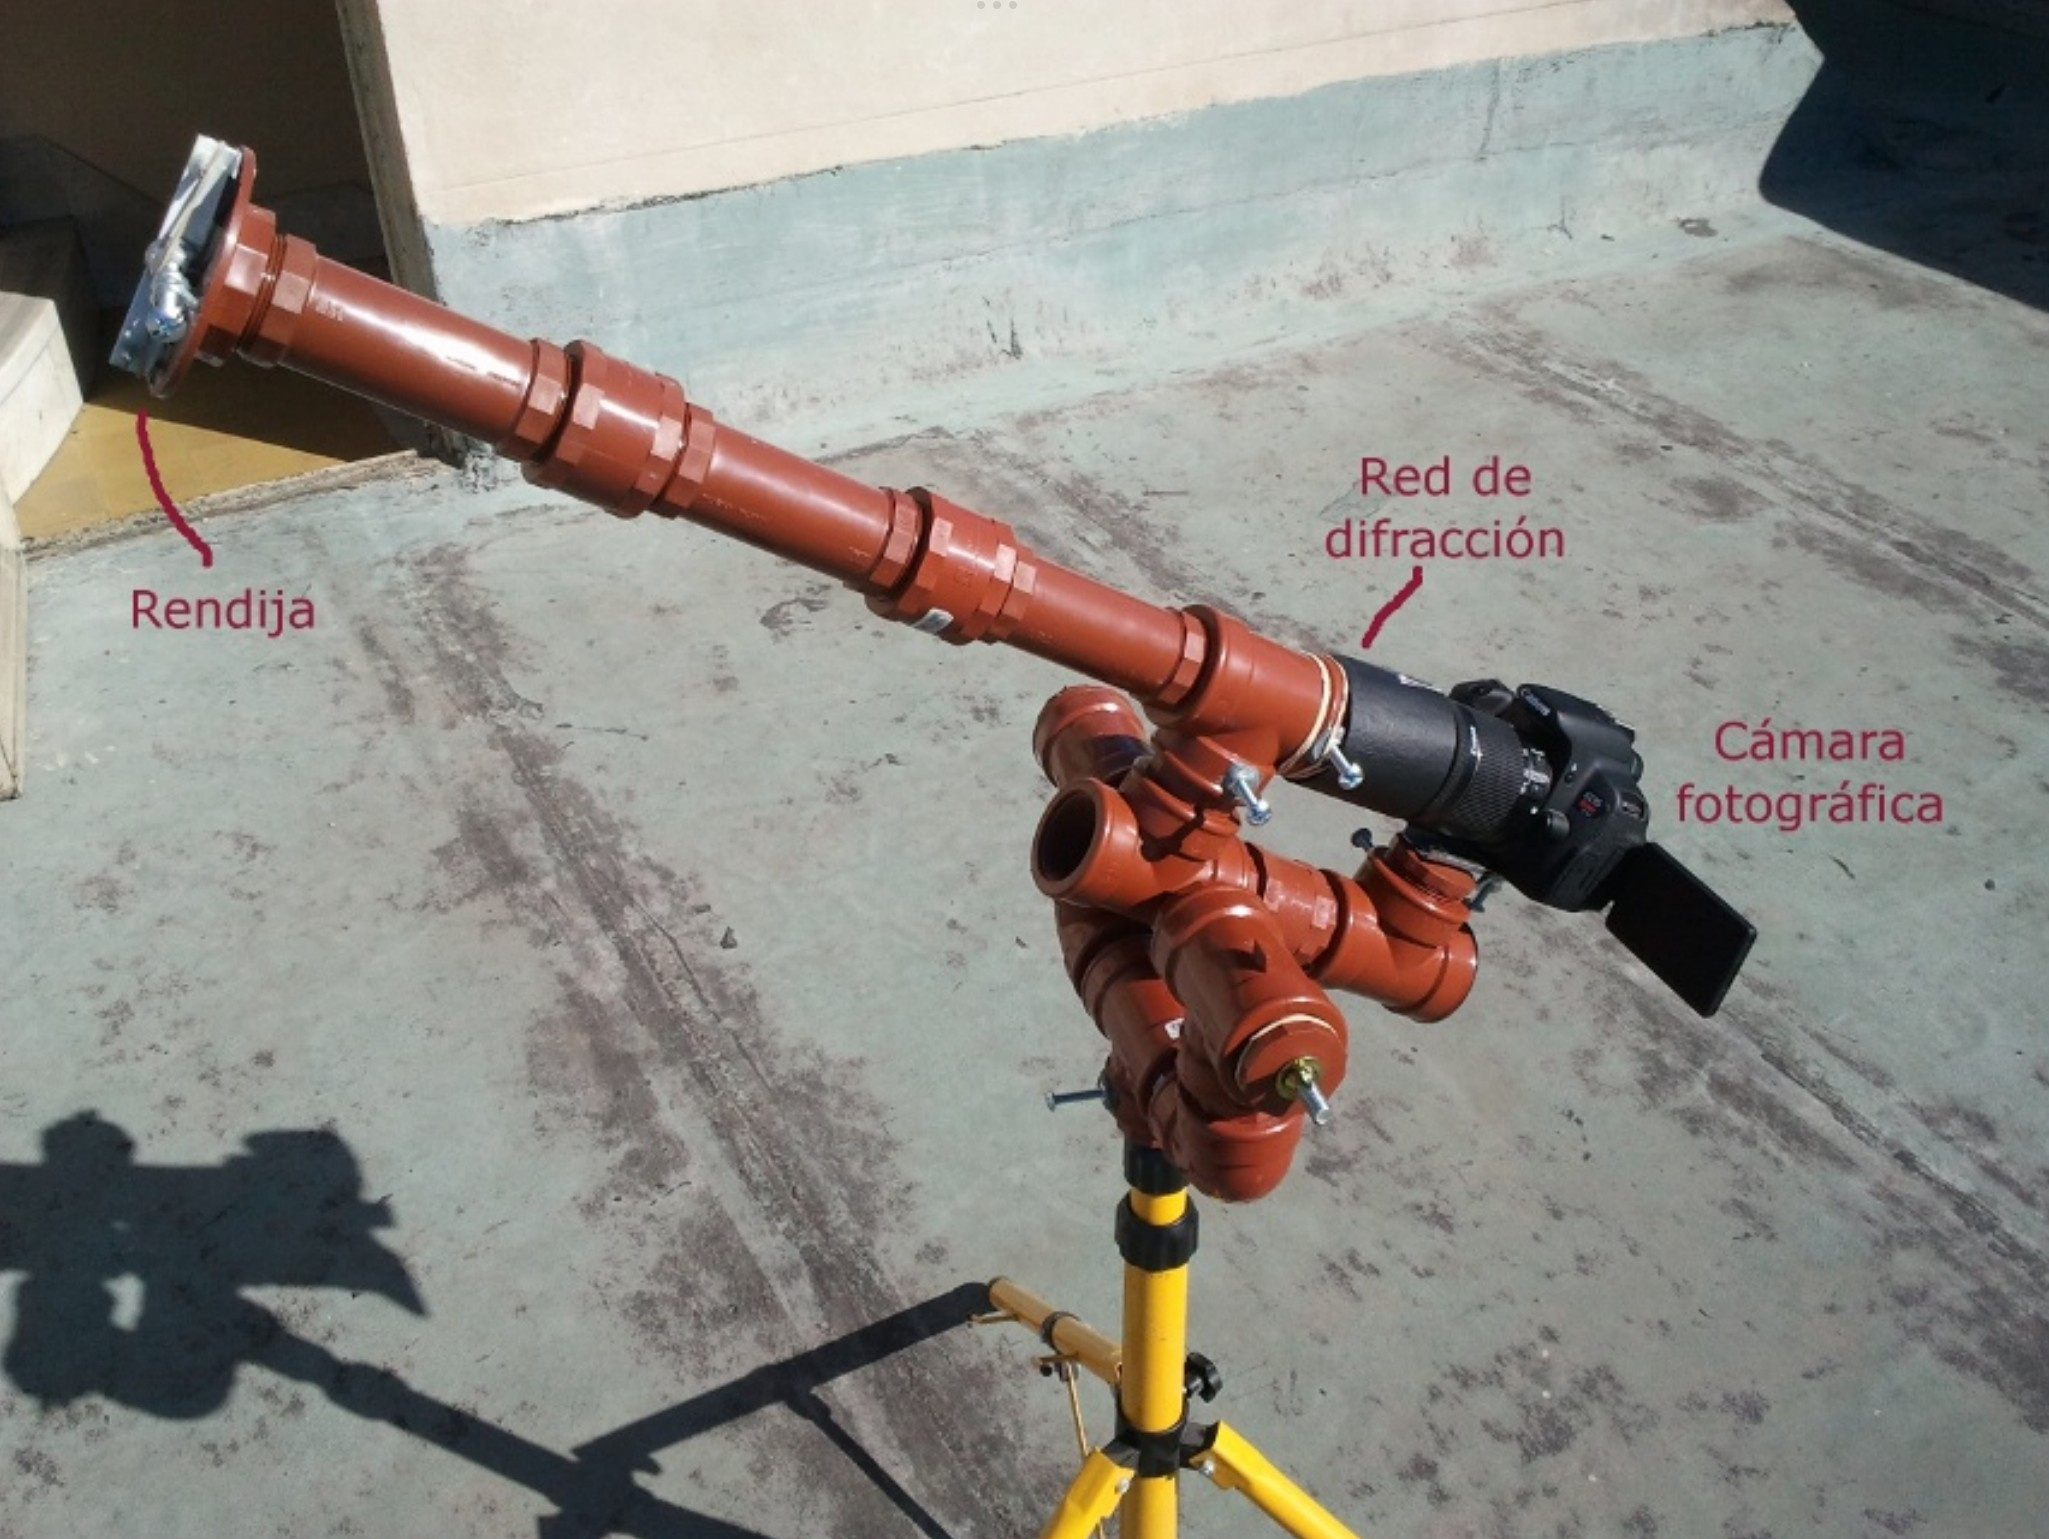
\includegraphics[width=.98 \linewidth]{images/Screenshot_2024-10-15-17-15-57-031_com.google.android.apps.docs~2.jpg}
    \caption{Espectro-caño-grafo}
    \label{espectrografo}
\end{wrapfigure}
Para la obtención del espectro visible, se utilizó un dispositivo llamado espectro-caño-grafo (Figura \ref{espectrografo}), el cual consistía en una cámara fotográfica y una red de difracción oculta dentro de un tubo oscuro, lo que nos permitió obtener el espectro visible de la luz del sol.


La imagen se tomó el día 6 de septiembre de 2024 a las 16:29hs en un día soleado sin nubes. La cámara se configuró con un ISO de 100, apertura de 7.0 con distancia focal de 55mm y tiempo de exposición 1/16 segundos. 
El objeto apuntado fue una pared de color beige.
La captura se realizó en formato RAW para asegurar la máxima calidad posible en la imagen.

Posteriormente, se trabajó con el espectro obtenido por medio del software llamado \textit{Fitswork} de Jens Dierks, que nos permitió realizar una serie de operaciones sin alterar la información de la imagen como: enderezarla, recortarla y pasarla a escala de grises que resaltaba los valores negros que representaban las lineas de absorción. El archivo editado se guardó en formato $.fit$ para seguir trabajando en el software \textit{Annie} de Luis Lopez. 

Una vez importado el archivo en \textit{Annie}, la aplicación lo tradujo a un gráfico de intensidades en función de posición en eje X (píxeles), por lo que era necesario calibrar la imagen para que sea un gráfico de intensidad en función de longitud de onda (en Ángstrom). En nuestro caso, pudimos identificar dos picos muy evidentes para ayudarnos en este proceso: Primer pico a la izquierda $x=183$ calibrado como 4861 $\AA$; Segundo pico elegido fue en $x=239$ calibrado como 5167 $\AA$. El espectro utilizado de referencia para la calibración fue el siguiente: \href{https://jazzistentialism.com/blog/wp-content/uploads/2014/05/fraunhoferlines.jpg}{Fraunhoferlines.jpg}. Para minimizar errores en este proceso de calibración, es mejor elegir dos líneas bien separadas en el espectro. Esto ayuda a que la calibración sea más precisa, ya que distribuye mejor cualquier pequeño error a lo largo de todo el gráfico. Además, facilita identificar con más exactitud la relación entre los píxeles de la imagen y las longitudes de onda reales. Si se usan líneas muy cercanas, el ajuste podría ser menos preciso en otras partes del espectro. Por eso, seleccionar puntos alejados asegura un resultado más confiable.

Una vez calibrado el espectro, identificamos manualmente los elementos presentes comparando las longitudes de onda de las líneas de absorción presentes con las longitudes de onda registrados en el \textit{Solar Flux Atlas (L. Wallace and K. Hinkle, 2011)}.

Para un mejor análisis, se comparó el espectro obtenido con las distintas clases espectrales para ver cual se asemeja más al nuestro. Luego, mediante la ley de Wien logramos despejar la temperatura aparente del sol, utilizando el dato obtenido del espectro de la longitud de onda en donde se registró una máxima intensidad. 

Posteriormente pudimos confeccionar un par de gráficos de acuerdo con la Ley de Planck y con la ayuda de un script en Python que nos brindaron los docentes a cargo y con datos espectrales de Thekaekara. 

Para finalizar realizamos un análisis comparativo entre los datos que obtuvimos por nuestra cuenta con los obtenidos por dos de nuestros compañeros, Francisco Apolo y Martin Dolinsky.

%%%%%%%%%%%%%%%%%%%%%%%%%%%%%%%%%%%%%
\section{Resultados y análisis}
\subsection{Elementos identificados}

\begin{figure}[H]
    \centering
    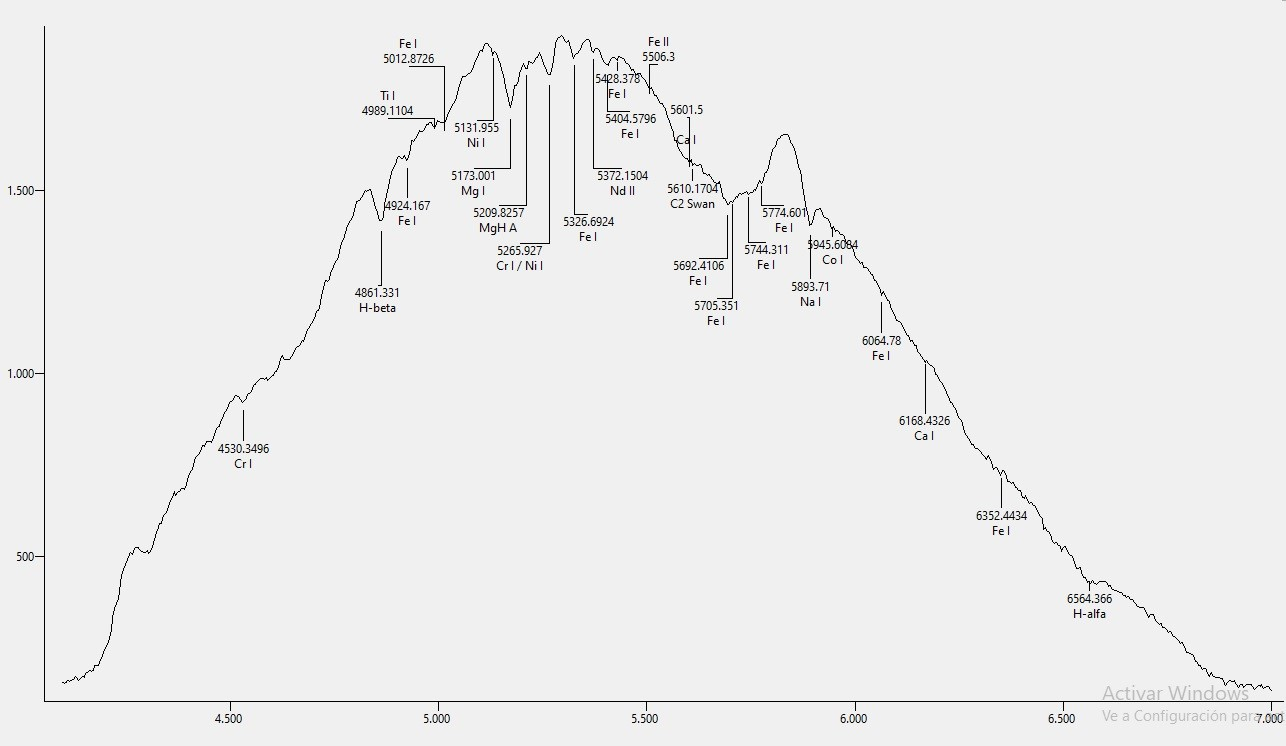
\includegraphics[width=1\linewidth]{images/grafico-elementos-completos.jpg}
    \captionsetup{justification=centering}
    \caption{Gráfico de intensidades en función de longitud de onda con elementos identificados}
    \label{fig:calibrado-con-elementos}
\end{figure}
El elemento predominante del gráfico observado en Figura \ref{fig:calibrado-con-elementos} es \textit{Fe I}, contando con 11 líneas de absorción identificadas. En menor cantidad, se habían identificado también otros elementos como \textit{Cr I}, \textit{Ti I}, \textit{Ni I}, \textit{Mg I}, \textit{MgH A},  \textit{Nd II}, \textit{Fe II}, \textit{Ca I}, \textit{Na I}, \textit{Co I}, \textit{H},  entre otros. 

La presencia de líneas predominantes de \textit{Fe I} indica que estamos observando las capas exteriores del Sol, donde los átomos de hierro permanecen neutros debido a las temperaturas más bajas en comparación con el núcleo. Esto, a su vez, nos permite inferir que el Sol se encuentra en una etapa de su evolución donde está fusionando hidrógeno en helio en su núcleo, un proceso característico de las estrellas de la secuencia principal.

También hay picos muy evidentes en $\lambda _1: 4861 \,\AA$, $\lambda _2: 5167 \,\AA$, ${\lambda _3: 5893,71 \,\AA}$ y $\lambda _4: 6563 \,\AA$ Identificados como $H \beta$, \textit{ Mg I}, \textit{Na I}, $H \alpha$ respectivamente.




\subsection{Temperatura}
\subsubsection{Análisis con clases espectrales A2V, G2V y M2V}
\begin{figure}[H]
    \centering
    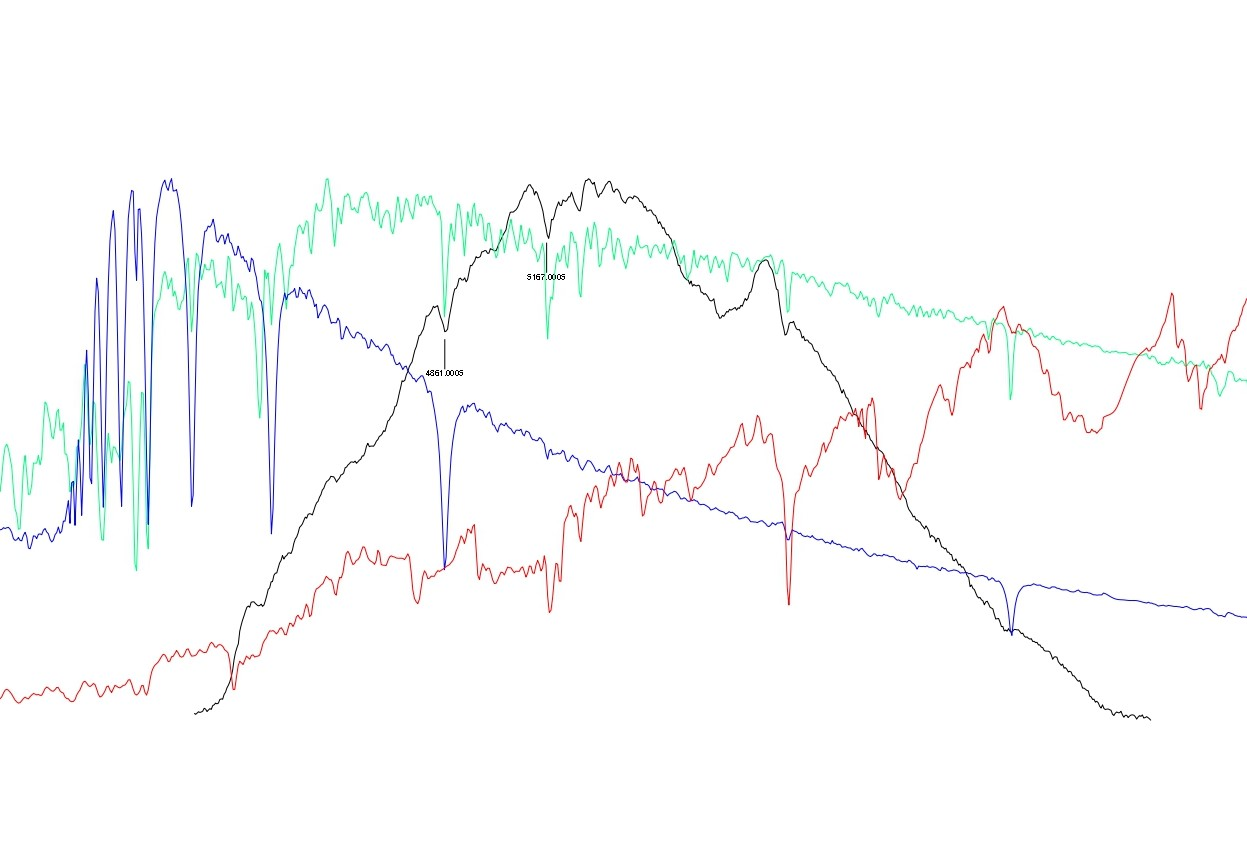
\includegraphics[width=1\linewidth]{images/comparacion_de_perfiles_forro_page-0001.jpg}
    \captionsetup{justification=centering}
    \caption{Gráfico de intensidad en función de longitud de onda comparado con clases espectrales A2V (azul), G2V (verde) y M2V (rojo)}
    \label{fig:calibrado-con-clases-espectrales}
\end{figure}

En la Figura \ref{fig:calibrado-con-clases-espectrales} se pueden observar espectros de distintas clases estelares: A2V, G2V y M2V. Las distintas clasificaciones dependen de la temperatura superficial de la estrella, siendo las de tipo O las más clientes y las M las más frías, siguiendo el orden O,B,A,F,G,K,M. 

Teniendo eso en cuenta se puede armar una tabla relacionando la clase espectral con el rango de la temperatura superficial. En nuestro caso consultamos la siguiente \href{http://hyperphysics.phy-astr.gsu.edu/hbasees/Starlog/staspe.html}{página}.


Se observa en Figura \ref{fig:calibrado-con-clases-espectrales} una notoria semejanza entre nuestro espectro y el del tipo G2V, lo cual tiene sentido porque el Sol pertenece a esta categoría de clase espectral G (estrellas amarillas). A partir de esta información podemos estimar una temperatura superficial de entre 5.000 - 6.000 K.  


\subsubsection{Ley de Wien}
Aplicando la ley de Wien, logramos despejar la temperatura aparente del sol en base a nuestros datos, la cual nos dio $5392,94 \pm 19.15$ K, tomando como lambda máxima $5377.4 \pm 19.1 \, \AA$. Este valor coincide con el valor que asumimos anteriormente, al decir que por ser una estrella de categoría G y que su temperatura variaba entre 5000 K y 6000 K.
Los cálculos realizados en esta sección se encuentran en Apéndice. 

\subsubsection{Ley de Planck}
Para el análisis de esta sección se utilizaron los datos proporcionados por el espectro de Thekaekara (año 1973) que se puede encontrar en el siguiente \href{https://www.nrel.gov/grid/solar-resource/assets/data/thekaekara.txt}{enlace}. También, los gráficos se realizaron mediante la librería de matplotlib en Python por medio de un \href{https://colab.research.google.com/drive/17XQ6ux3qzL6OkIsI6bAN3YS1U75l0VIM?usp=sharing}{programa} proporcionado por los docentes. 

\begin{figure}[H]
    \centering
    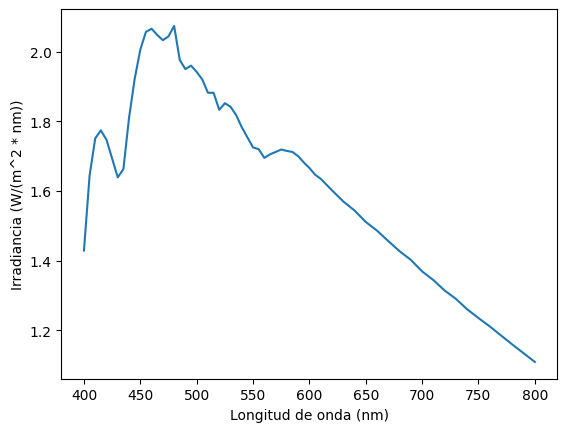
\includegraphics[width=1\linewidth]{images/Copy of grafico_simple_planck.png}
    \captionsetup{justification=centering}
    \caption{Gráfico de irradiación $(W/(m^2*nm))$ en función de longitud de onda $(nm)$}
    \label{fig:planck-1}
\end{figure}

Este gráfico de Figura \ref{fig:planck-1} es distinto al que obtuvimos nosotros ya que el nuestro se trataba de la intensidad en función de longitud de onda mientras que este trata de la irradiancia en función de longitud de onda. 

Pero, a pesar de esa diferencia, podemos observar algunas similitudes ya que tanto la irradiancia como la intensidad son unidades de energía. Podemos ver por ejemplo los picos más evidentes que se encuentran aproximadamente en las mismas posiciones de longitudes de onda como en $\lambda _1 \approx 450 nm$ y $\lambda _2 \approx 550 nm$.

También, se puede apreciar que los valores obtenidos de longitud de onda tiene un rango mayor al obtenido por nosotros mediante nuestra cámara y junto al caño-espectrógrafo. Nosotros con los instrumentos disponibles mencionados anteriormente, pudimos interceptar longitudes de onda entre 410 nm y 700 nm aproximadamente (visto desde el gráfico de Figura \ref{fig:calibrado-con-elementos} y a partir del recorte de la imagen original). En cambio, en este archivo de Thekaekara, se registró longitudes de onda de entre 115 nm y 400000 nm (aunque en el script de Python acota el rango de 400nm a 800nm). El señor \href{https://en.wikipedia.org/wiki/Matthew_Pothen_Thekaekara}{Thekaekara} (1914-1976) quien fue un científico indio especializado en espectrofotometría, probablemente tuvo mejores instrumentos de medición que nosotros y un conocimiento más amplio sobre el tema para capturar los datos en las mejores condiciones. 
Además, nosotros cuando capturamos el espectro no tuvimos en cuenta la interferencia generada por la atmósfera terrestre, ya que ésta puede añadir más líneas de absorción que no son del espectro solar, y  reflejar ciertas longitudes de onda dependiendo el ángulo de incidencia del rayo solar en la atmósfera en ese momento (Ley de Snell).

\begin{figure}[H]
    \centering
    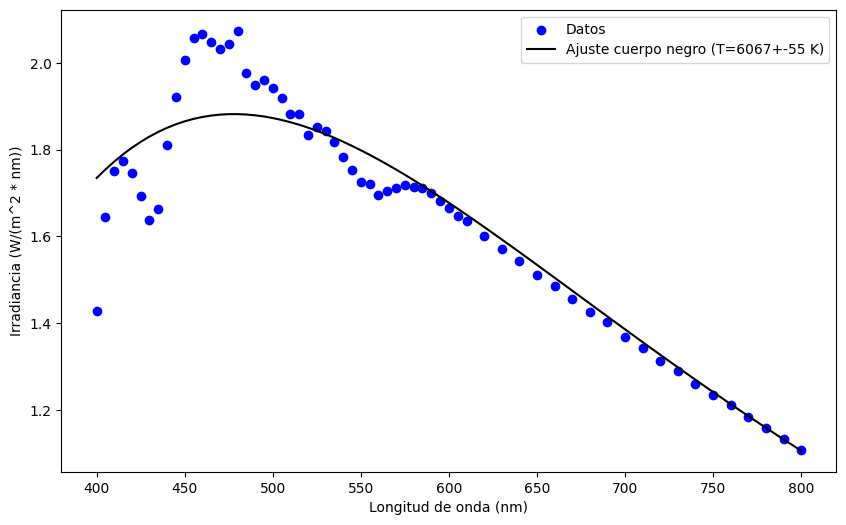
\includegraphics[width=1\linewidth]{images/Copy of grafico_con_ajuste_planck.png}
    \captionsetup{justification=centering}
    \caption{Gráfico de irradiación $(W/(m^2*nm))$ en función de longitud de onda (nm) con curva de ajuste de cuerpo negro (en negro)}
    \label{fig:planck-2}
\end{figure}

En esta figura se presentan fragmentados los mismos datos que el en grafico anterior (Figura \ref{fig:planck-1}) junto con una curva obtenida por el ajuste de cuerpo negro mediante la Ley de Planck y los valores de longitud de onda del mismo archivo.

Se observa que el ajuste del cuerpo negro se asemeja a los datos obtenidos entre los 500 nm y los 800 nm. Esto puede deberse a varios factores. El primero puede ser que un cuerpo negro es una figura ideal (un modelo), por lo que no existe realmente, y por lo tanto los resultados son una aproximación. Otro puede ser que la superficie del sol no es homogénea, por lo que en distintos sectores va a presentar distinta concentración de elementos y va a emitir distintas longitudes de onda. 


\subsection{Análisis Comparativo}
\begin{figure}[H]
    \centering
    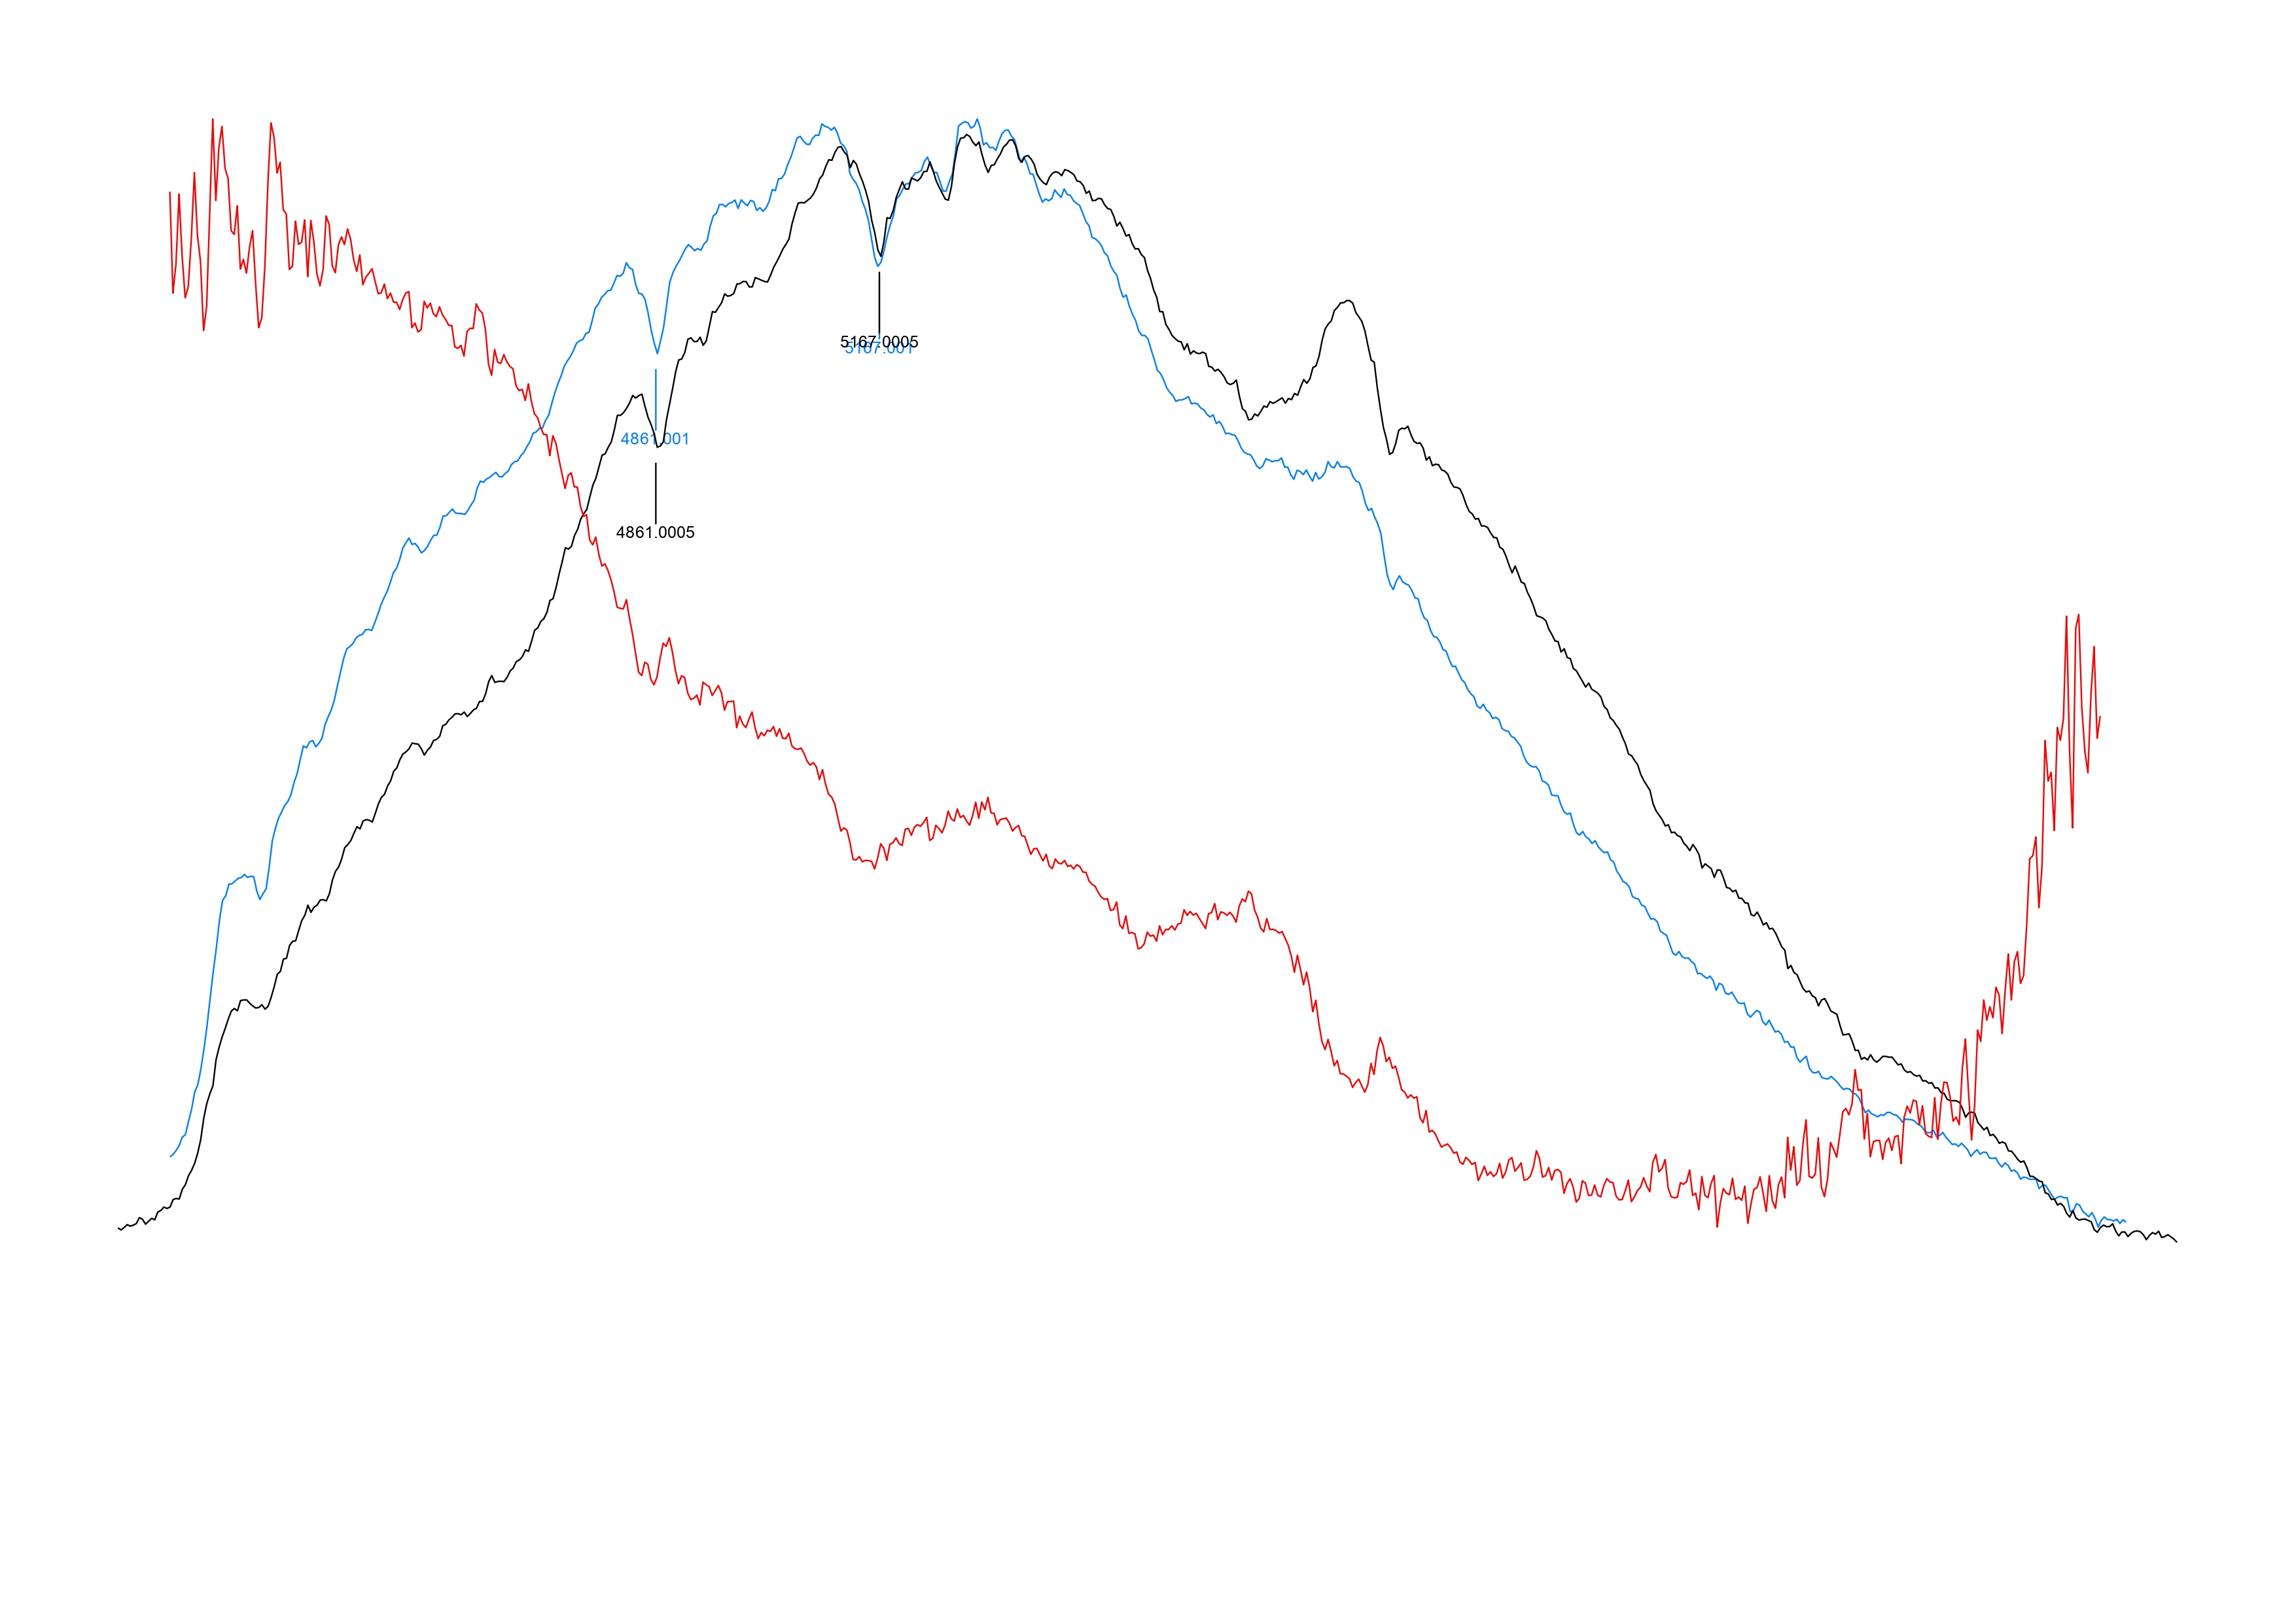
\includegraphics[width=1\linewidth]{images/division_perfiles_page-0001.jpg}
    \captionsetup{justification=centering}
    \caption{Gráfico comparativo de las curvas de intensidad en función de longitud de onda obtenidos por nosotros (negro), los obtenidos por otro grupo (azul) y la división de las dos curvas (rojo)}
    \label{fig:graf-comparativo}
\end{figure}

Primero que nada cabe destacar que ambos gráficos son muy similares, ya que los datos fueron recopilados en circunstancias parecidas, con los mismos instrumentos y desde el mismo punto de observación. Se pueden identificar casi los mismos picos en las dos curvas (negra y azul). 

La principal diferencia entre las curvas que obtuvimos y la que obtuvo el otro grupo es el valor de la intensidad, y esto se debe por las distintas configuraciones de la cámara durante la captura de la imagen; un mayor tiempo de exposición resulta en una mayor intensidad en la curva.

La curva roja es la división entre ambas curvas, siendo la azul el divisor  y la negra el dividendo. En una operación matemática como la división, cuando el divisor es mayor que el dividendo los valores tienden a ser más grandes, y por el contrario cuando se intervienen los roles, los valores tienden a 0. Se puede notar que al principio comienza en la parte superior de la imagen, ya que la curva azul tenía mayor intensidad que la curva negra en esas longitudes de onda. Mientras que en el centro tiene menos pendiente la curva ya que tanto el azul y el negro se asemejan en esos valores. Y finalmente, como la curva negra es mayor que el azul, la curva roja continúa siendo decreciente salvo en el último tramo donde la curva negra vuelve a ser menor y que el azul y la curva roja se vuelve creciente nuevamente. 

Una observación muy interesante en relación al análisis del párrafo anterior es que la diferencia de la curva negra y la curva azulada es similar o parecido tanto en el lado derecho e izquierdo del gráfico, tomando de centro donde las dos curvas coinciden en intensidad. Esto muestra que obtuvimos más intensidad para las longitudes de onda más largas (rojas) mientras que el otro grupo obtuvo más intensidad para las longitudes de onda más cortas (azules). 


\section{Conclusiones}
Durante el desarrollo de este trabajo quedó en evidencia toda la información que se puede obtener desglosando el espectro visible de la luz que nos llega desde el sol; información como su temperatura o incluso de los elementos con los que está compuesto.

La identificación de líneas de absorción, como las de \textit{Fe I}, \textit{Mg I}, \textit{Na I} y \textit{H}, refleja la complejidad de la composición de las capas exteriores del sol. Además, la aplicación de la Ley de Wien permitió calcular una temperatura coherente con la categoría espectral G2V, validando nuestras mediciones experimentales.

Durante el ajuste mediante la Ley de Planck nos mostró las limitaciones de los modelos ideales. También, las diferencias entre nuestros datos y los del archivo de Thekaekara subrayan la importancia de realizar observaciones en condiciones óptimas, como fuera de la atmósfera ya que en este caso podría interferir en el resultado añadiendo más líneas de absorción y reflejando parte del espectro.

Asimismo, la comparación con datos obtenidos por otro grupo refleja cómo las configuraciones de los instrumentos pueden influir en los resultados, destacando la necesidad de calibraciones precisas. Este trabajo también nos demostró que la experimentación casera, si bien limitada en alcance, puede ofrecer resultados significativos y comparables con observaciones más profesionales.

Para finalizar, este trabajo práctico nos permitió entender mejor cómo la temperatura y la composición química determinan las características espectrales. Sabiendo todo esto, nos posibilita aplicar las mismas técnicas para estudiar estrellas con características similares al sol y de su respectiva evolución, con el fin de comprender y conocer más nuestro universo.

\newpage

%-----------------------
\section{Apéndice}
\subsection{Ley de Wien}
\subsubsection{Hallar parametros de longitudes de onda}
Hallar $\Delta \lambda$ con $\lambda_1=5396,5 \, \AA$ y $\lambda_2=5358,3 \, \AA$
 \begin{align}
     \Delta \lambda = \frac{\lambda_1 - \lambda_2}{2} = \frac{5396,5 \AA - 5358,3 \AA}{2} = 19,1 \AA
 \end{align}
Hallar $\lambda _{max}$ con $\lambda _1$ y $\Delta \lambda$, donde $\lambda _{max}$ es punto medio entre $\lambda _1$ y $\lambda _2$
\begin{align}
    \lambda _{max} = \lambda _1 - \Delta \lambda = 5396,5 \AA - 19,1 \AA = 5377,4 \AA
\end{align}

\subsubsection{Hallar valores de temperatura}
Hallar temperatura con $\lambda _{max}$
\begin{align}
    T = \frac{2,9 \times 10^{-3}m \, \text{K}}{\lambda _{max}} = \frac{2,9 \times 10^{-3}m \,K}{5377,4 \times 10^{-10}m} = 5392,94 \, \text{K}
\end{align}
Hallar incerteza de temperatura $\Delta T$
\begin{align}
    \Delta T &= \left | \frac{d T}{d \lambda} \right | \Delta \lambda \\
    \Delta T &= \frac{2,9 \times \10^{-3}m \, K}{\lambda ^2} \Delta \lambda \\ 
    \Delta T &= \frac{2,9 \times \10^{-3}m \, K}{(5377,4 \times 10^{-10}m)^2} \times 19,1 \AA = 19,15 \, \text{K}
\end{align}

%%%%%%%%%%%%%%%%%%%%%%%%%%%
\vspace{0.1cm}
\hline
\vspace{0.1cm}
\section{Bibliografia y referencias}
\begin{itemize}
    \item \textit{Solar Flux Atlas for the Visible and Near Infrared (L. Wallace and K. Hinkle, 2011)} \url{https://drive.google.com/file/d/12cb7878UPS4j_bLrp3BIeYz9CMK9gR8b/view}
    \item \textit{Fraunhofer lines} \url{https://jazzistentialism.com/blog/wp-content/uploads/2014/05/fraunhoferlines.jpg}
    \item \textit{Tipos espectrales de estrellas} \url{http://hyperphysics.phy-astr.gsu.edu/hbasees/Starlog/staspe.html}
    \item \textit{Script de Python para ajuste de cuerpo negro (Ley de Planck)} \url{https://colab.research.google.com/drive/17XQ6ux3qzL6OkIsI6bAN3YS1U75l0VIM?usp=sharing}
\end{itemize}

\end{document}
